\chapter{Measures that answer different questions}\label{ch:measures}

Most disclosure assessments end in a table, and most such tables have a row headed
``re-identification risk''. Readers of these tables, careful ones included, tend to
bring one belief to that row. They take the measures in circulation, the prosecutor
risk, the journalist risk, the marketer risk, the share of sample-unique records and
the reciprocal of a key frequency, to be different summaries of one underlying
quantity. On this view the measures should roughly agree, an analyst may report
whichever suits the release, and a cautious analyst can quote the largest and be safe.

The belief deserves a fair statement, because it has real support. Every one of these
measures is computed from the same key frequencies. Each is a number between zero and
one that is read as a probability. Each falls when key classes grow and rises when they
shrink, so across two releases they usually rank the files in the same order. The
handbooks present them together \citep{hundepool2012}, and software prints them side by
side. Measures that move together and share a vocabulary look like views of one thing.

The first fact that breaks the belief is a single release. On the synthetic register
used throughout this book, a population of 200,000 units from which a 5 per cent
sample is released, the mean prosecutor risk of the unprotected release is 0.466.
% source: paper/generated/numbers.tex (\runprosecutormean, \runpopulation)
The same mean computed with population frequencies in place of sample frequencies is
0.064, and the marketer risk for an adversary who does not know who is in the file is
0.023.
% source: paper/generated/numbers.tex (\runpluginpopulation, \runmarketerunconditional)
These are three figures for one file, one key and one adversary's knowledge, and the
largest is twenty times the smallest.
% source: paper/generated/numbers.tex (\rununconditionalratio)
None of them is a computing error. A factor of twenty separates a figure that most
release committees would accept from one that none would. The rule of quoting the
largest fails as well, for a reason this chapter reaches near its end: the largest of
these measures is not an upper bound on anything once the adversary knows more than the
key.

This chapter therefore asks one question. What experiment does each measure describe,
and when can a figure computed for one experiment stand in for a figure computed for
another?

\section{Three records of one release}

The question first reached the Bank as an audit finding. Grace, from internal audit,
had been asked to check that the Bank's past release decisions could be reproduced from
their records. She pulled the files for three products drawn from the same household
survey: a public extract, a scientific-use file for accredited researchers, and a
tabular release. All three records reported a ``re-identification risk'', and all three
cited a tolerance. Grace could reproduce none of the figures from the records alone,
because none of them said whether the target was assumed to be in the file, whose
frequencies had been used, or whether the sampling fraction had been applied.

Naledi, the Bank's disclosure control officer, recomputed each figure from the archived
data and found that the three records had used three different quantities under one
name. Her note to the chair of the release committee was short. The measures were not
three estimates of one risk. They were the answers to three different experiments, and
the records had not said which experiment each answered. The rest of this chapter
follows the argument her note had to make.

\section{Three experiments on one file}

Chapter~\ref{ch:scenario} defined a disclosure risk as the probability of one
experiment: a declared adversary, holding declared information about a target, applies
a linkage rule to the release, and succeeds when it names the target's record. The
names prosecutor, journalist and marketer, which \citet{elemam2008} gave to three
conventional scenarios, are labels for three such experiments. They differ in two
choices that the adversary's position fixes before any data are seen. The first choice
is whether the adversary knows that the target is in the file. The second is whether the
adversary attacks one target or many.

The \emph{prosecutor} knows that the target is in the released file, perhaps because the
target told someone that they took part in the survey, or because the file is a census
of a population the target is known to belong to. Under the four assumptions of
Proposition~\ref{prop:recip}, its chance of naming a target whose key is $k$ is
$1/f_k$, where $f_k$ is the number of released records with that key. The file-level
summaries are the mean of $1/f_k$ over released records, which describes a target drawn
uniformly from the file, and the maximum, which describes the worst released record.

The \emph{journalist} does not know whether the target is in the file. It starts from a
released record that looks rare and asks whether that record can be tied to one person
in the population. The quantity that decides this is the population frequency $F_k$ of
the record's key, which the journalist cannot see in the release.

The \emph{marketer} attacks many targets at once and values the share it links
correctly. Its risk is an average over a declared population of targets. Whether that
population is the released file or the whole population, and whether the marketer knows
which units are in the file, are two further choices, and each changes the figure.

Figure~\ref{c03:fig-measures} places the ten summaries that the simulation study
computes for the unprotected release on one logarithmic axis and groups them by the
experiment they describe. The axis runs over three orders of magnitude. The bars with
the same shade and hatch belong to the same experiment, and within each group the
figures agree with one another or differ for a stated reason. Between groups they
differ by factors from two to more than a hundred. The sections below take the groups in
turn.

\begin{figure}[t]
\centering
% source: paper/generated/table_measures.tex (all ten values)
\begin{tikzpicture}
\begin{axis}[
  xbar, bar width=7pt, width=0.80\textwidth, height=8.6cm,
  xmode=log, log origin=infty, xmin=0.001, xmax=1.5,
  xlabel={Value of the summary (logarithmic scale)},
  ymin=0.4, ymax=10.6,
  ytick={1,2,3,4,5,6,7,8,9,10},
  yticklabels={Naive $\pi$ used as risk, $\rho$ model-based, $\rho$ truth,
    $\pi$ times plug-in, Marketer unconditional, Plug-in $1/F_k$,
    Share with $f_k=1$, Prosecutor maximum, Marketer $D_I/n$, Prosecutor mean $1/f_k$},
  y tick label style={font=\footnotesize}, x tick label style={font=\footnotesize},
  xlabel style={font=\footnotesize},
  legend style={font=\footnotesize, at={(0.5,-0.2)}, anchor=north, legend columns=2,
    draw=none},
  legend cell align=left,
  area legend]
\addplot[bar shift=0pt, draw=black, fill=gray!20, postaction={pattern=north east lines}]
  coordinates {(0.4663,10) (0.4663,9) (1.0,8) (0.2719,7)};
\addlegendentry{Target in file, released candidates}
\addplot[bar shift=0pt, draw=black, fill=gray!50, postaction={pattern=horizontal lines}]
  coordinates {(0.0636,6)};
\addlegendentry{Population frequencies known}
\addplot[bar shift=0pt, draw=black, fill=gray!75, postaction={pattern=crosshatch}]
  coordinates {(0.0233,5)};
\addlegendentry{Membership unknown}
\addplot[bar shift=0pt, draw=black, fill=white, postaction={pattern=crosshatch dots}]
  coordinates {(0.0032,4)};
\addlegendentry{No experiment}
\addplot[bar shift=0pt, draw=black, fill=gray!35, postaction={pattern=vertical lines}]
  coordinates {(0.0227,3) (0.0274,2) (0.05,1)};
\addlegendentry{Uniqueness probability}
\end{axis}
\end{tikzpicture}
\caption{Ten summaries of one synthetic release ($N = 200{,}000$, $\pi = 0.05$,
$n = 10{,}035$), grouped by the experiment each describes. Shade and hatch mark the
group. The axis is logarithmic, so equal distances are equal ratios.}
\label{c03:fig-measures}
\end{figure}

\section{The prosecutor and an identity}

Start with the group at the top of Figure~\ref{c03:fig-measures}, where the target is
known to be in the file and the adversary chooses among released candidates. Two of its
bars have the same length, 0.4663, and that is no coincidence.
% source: paper/generated/table_measures.tex
The mean prosecutor risk over released records and the marketer risk computed as the
number of distinct released keys divided by the number of released records are the same
quantity.

\begin{proposition}[The in-file marketer identity]\label{c03:prop-ident}
Let $D_I$ be the number of distinct keys among the $n$ released records. Under
Assumptions~\ref{as:key} to~\ref{as:unif},
\begin{equation}\label{c03:eq-ident}
\frac{1}{n}\sum_{i \in I}\frac{1}{f_{K_a(X_i)}} = \frac{D_I}{n}.
\end{equation}
\end{proposition}

The identity holds because each occupied key class contributes $f_k$ records, each with
risk $1/f_k$, and so contributes exactly one to the sum. It has a plain reading. A
marketer who attacks every released record and picks uniformly within each key class
gets one correct link per class on average, so its expected haul is the number of
classes. On the synthetic release there are 4,679 distinct keys among 10,035 records,
% source: paper/generated/numbers.tex (\runreleasedcells, \runreleased)
which gives the figure in the first two bars. The identity also gives a check on
software: a program that reports a mean prosecutor risk different from $D_I/n$ on an
unperturbed release has an error somewhere.

The other two bars in the group summarise the same distribution differently. The
maximum prosecutor risk is 1, because 27.2 per cent of the released records are unique
in the sample.
% source: paper/generated/numbers.tex (\runreleaseduniqueshare); table_measures.tex
A maximum of 1 says that at least one record is fully exposed to a prosecutor. It says nothing about how many, which is what the share of sample uniques adds. A
committee that receives the whole distribution of $1/f_k$ across released records can
read both summaries from it, and more besides.

The prosecutor figures carry a condition that the label hides. The value $1/f_k$ is the
success probability only under the four assumptions of Proposition~\ref{prop:recip}:
an unperturbed key, an adversary that observes the key without error, records that are
exchangeable within the key class, and a uniform choice among them. Chapter~\ref{ch:scenario} showed that the third assumption fails whenever the adversary holds a reading of a released
variable outside the key, and that in that case the success probability can exceed
$1/f_k$. The prosecutor maximum is then the largest value of a formula, not the largest
risk. This is why the cautious rule of quoting the largest measure fails. The largest
measure in the table is computed under assumptions that an informed adversary breaks,
so it bounds only the risk of an uninformed one.

The public record shows how easily an adversary comes to know that a target is in a
file. In the case reported by \citet{sweeney2002}, a state agency released hospital
records of state employees and their families with names removed. The file covered a
defined group, so anyone who knew that a person belonged to the group and had been
treated knew that the person's record was in it. Sweeney identified the record of the
state governor by his date of birth, sex and postcode. Whoever holds that kind of
knowledge is a prosecutor in the sense of this section, and a file in which those three
attributes leave most records alone in their key class gives it little protection.

\section{Sample and population frequencies}

The second group in Figure~\ref{c03:fig-measures} holds one bar, the mean of $1/F_k$
over released records, where $F_k$ is the population frequency of the record's key. Its
value is 0.064, against 0.466 for the same mean with sample frequencies, a ratio of
7.3.
% source: paper/generated/numbers.tex (\runpluginpopulation, \runprosecutormean, \runpluginratio)
Both figures have been published as the re-identification risk of a file, and an
analyst who did not know which had been computed could not tell from the number alone.

The two figures describe different experiments. The mean of $1/f_k$ describes an
adversary choosing among released candidates. The mean of $1/F_k$ describes an
adversary who starts from a released record and must find its owner among all members of
the population with the same key, as one would by searching a full population list for
the record's combination of attributes. The second experiment is the one behind the
second step of that case, where the released record was matched against the voter list
of the governor's town \citep{sweeney2002}. Sweeney's estimate that simple demographics identify most
of the United States population \citep{sweeney2000}, revisited with later census data by
\citet{golle2006}, is a statement about population frequencies: it counts how often
$F_k = 1$. Neither experiment is more correct than the other. They answer different
questions.

What can be said in general is the sign of the gap. Since the released sample is a
subset of the population, no key class can have more members in the sample than in the
population, and so the sample-frequency measure can never fall below the
population-frequency measure.

\begin{proposition}[Ordering and plug-in bias]\label{c03:prop-plugin}
For every key $k$ with $f_k > 0$, $1/f_k \ge 1/F_k$ pathwise, so for every released
record $i$,
\begin{equation}\label{c03:eq-order}
\E\Big[\frac{1}{f_{K(i)}}\Big] \ \ge\ \E\Big[\frac{1}{F_{K(i)}}\Big],
\end{equation}
with equality only if every member of every occupied key class is in the sample. If
$f_k$ is positive with probability one and has finite mean, then
\begin{equation}\label{c03:eq-jensen}
\E\Big[\frac{1}{f_k}\Big] \ \ge\ \frac{1}{\E[f_k]},
\end{equation}
strictly unless $f_k$ is degenerate.
\end{proposition}

The first part fixes the direction of the error when one frequency is used in place of
the other. An analyst who has population frequencies to hand and reports the mean of
$1/F_k$ for an adversary who in fact chooses among released candidates understates that
adversary's success, and by a factor that can be large: on the synthetic release it is
7.3. The reverse substitution overstates. The direction is known before any data are
seen, and that is useful, because a reviewer can tell from the description alone which
way a mislabelled figure errs.

The second part concerns a different shortcut. Some reports compute the average key
frequency and quote its reciprocal as the risk, on the reasoning that a typical record
shares its key with that many others. By Jensen's inequality the reciprocal of an
average frequency is never larger than the average of the reciprocal frequencies. On the
synthetic release, where the mean sample frequency of a released record's key class
gives a reciprocal of 0.191, the shortcut reports less than half of the mean prosecutor
risk of 0.466.
% source: artifacts-paper/results.json (measures.plugin_ordering.reciprocal_of_mean = 0.1914)
The reason is that rare keys carry most of the risk, and an average frequency is
dominated by the common ones. A reciprocal-of-average figure is therefore biased
downwards for the in-file experiment, with a known sign, and it should not appear in a
decision record as a risk.

At the Bank, this was the substance of the first finding. The scientific-use file of
the earlier record had been assessed with population frequencies taken from the census,
because the census was available and seemed the more complete source. The researchers
who would receive the file, however, would be choosing among released records. Naledi's
recomputation put the in-file risk at several times the recorded figure, and the record had compared the smaller figure with the tolerance.

\begin{example}[Five figures for an eight-record file]\label{c3:ex-five}
Before the committee met again, Grace asked Naledi for a file small enough that every member could check each figure by hand. The example below is the one Naledi gave her, and it carries each of the figures discussed so far. A population of 40 units falls into five key classes with population frequencies $F_A=12$, $F_B=10$, $F_C=3$, $F_D=5$ and $F_E=10$. A sample of eight is released, so $\pi=0.2$, and its keys are A, A, A, B, B, C, D and E, with sample frequencies 3, 2, 1, 1 and 1. The mean prosecutor risk is $(3\times\frac13+2\times\frac12+3\times1)/8=0.625$. The file has five distinct keys among eight records, and $D_I/n=5/8=0.625$, as Proposition~\ref{c03:prop-ident} requires. Three records are sample unique, so the prosecutor maximum is 1. With population frequencies the mean is $(3/12+2/10+1/3+1/5+1/10)/8=0.135$, and the in-file figure is $4.6$ times larger, in the direction Proposition~\ref{c03:prop-plugin} fixes. The mean sample frequency of a record's class is 2, and its reciprocal, $0.5$, falls below $0.625$, as Jensen's inequality says it must. The unconditional marketer risk is $0.2\times0.625=0.125$. Multiplying the population-frequency mean by $\pi$ gives $0.027$, the figure that answers no experiment.
\end{example}

\section{When membership is unknown}

The third group in Figure~\ref{c03:fig-measures} holds the marketer who does not know
which population units are in the file. Its risk is the unconditional risk of
Definition~\ref{def:risk}, averaged over a declared population of targets. By the
multiplication rule \eqref{eq:factor}, each target's unconditional risk is its inclusion
probability times its in-file risk. Under a common inclusion probability $\pi$ and exact
exchangeable matching the file-level figure is $\pi$ times the mean prosecutor risk, and
on the synthetic release that is $0.05 \times 0.4663 = 0.0233$.
% source: paper/generated/table_measures.tex (0.4663, 0.0233); numbers.tex (\runmarketerunconditional)
This figure is correct for its experiment, which is an adversary who draws a target from
the population without knowing whether that target was sampled. Its smallness is real:
in nineteen of every twenty attempts there is no record to find.

The fourth group holds a figure that answers no experiment, and it appears in the table
because reports have used it. It multiplies the population-frequency measure by the
sampling fraction, giving 0.0032.
% source: paper/generated/table_measures.tex
The product discounts for non-membership twice. The population frequency $F_k$ already
counts all the population members who share the key, sampled or not, so an adversary
choosing among them is already paying for not knowing who is in the file. Multiplying
by $\pi$ then charges for the same ignorance a second time. The result is less than one
per cent of the in-file figure and about a seventh of the correct unconditional one,
and it has no adversary behind it.
% arithmetic on table_measures.tex values: 0.0032/0.4663 = 0.007; 0.0032/0.0233 = 0.14

The two figures of the third and fourth groups show how a sampling fraction enters a
risk figure silently. In Grace's sample of past records, the public extract had been
assessed at 0.023, and the record compared that figure with a tolerance of 0.05 without
mentioning $\pi$. The figure was the right one for an adversary who did not know who was
sampled. It was the wrong one for the adversary the release committee had in mind, a
neighbour or a journalist who knew that a particular household had been interviewed,
for whom the factor of $\pi$ does not apply. The chair's question, when Naledi presented
the finding, was which adversary the committee had meant. The record did not say.

\section{The journalist and the uniqueness probability}

The last group in Figure~\ref{c03:fig-measures} belongs to the journalist, and it is
the one group that needs a model for something no one can observe. The journalist looks
at a released record that is unique in the sample, $f_k = 1$, and asks whether the
person behind it is also unique in the population. The classical object, studied by
\citet{skinnerholmes1998} and \citet{skinner2002}, is the probability that a sample
unique is a population unique,
\begin{equation}\label{c03:eq-rhodef}
\rho_k = \Prob(F_k = 1 \mid f_k = 1).
\end{equation}
It is not quite the journalist's success probability. A journalist who finds that the
record's key is shared by $F_k$ people in the population and picks one of them at random
succeeds with probability $1/F_k$, and averaging over what it does not know gives
$\E[1/F_k \mid f_k = 1]$, which is at least $\rho_k$. It differs again from the
journalist risk $1/\min_k F_k$ of \citet{elemam2008}, which is a worst case over key
classes. The three are close in a large population with many uniques and can be far
apart otherwise, which is reason enough to state which one a report contains.

\begin{proposition}[The uniqueness probability under Bernoulli sampling]\label{c03:prop-rho}
Suppose each population unit enters the sample independently with probability $\pi$,
and let $g(v) = \Prob(F_k = v)$ for $v \ge 1$ be the law of the population frequency of a
key class. Then
\begin{equation}\label{c03:eq-rho}
\rho_k = \frac{\pi\, g(1)}{\sum_{v \ge 1} v\pi(1-\pi)^{v-1} g(v)},
\end{equation}
and the journalist's success probability for a sample unique satisfies
\begin{equation}\label{c03:eq-journ}
\E\Big[\frac{1}{F_k}\ \Big|\ f_k = 1\Big] \ \ge\ \rho_k .
\end{equation}
\end{proposition}

Equation~\eqref{c03:eq-rho} shows what the sampling fraction contributes and what it
does not. It enters through the chance that a class of size $v$ leaves exactly one
member in the sample, which is $v\pi(1-\pi)^{v-1}$. The law $g$ of the population
frequencies enters as well, and $\pi$ alone does not determine $\rho_k$. Practice
sometimes reports $\pi$ itself as the journalist risk, on the reasoning that a
population unique is caught in the sample with probability $\pi$. That reasoning
computes the wrong conditional probability: it is the chance that a population unique
is sampled, not the chance that a sample unique is a population unique. On the
synthetic register the true value of $\rho$ at $\pi = 0.05$ is 0.0227, so using $\pi$
overstates it by a factor of 2.20, and at $\pi = 0.5$ by a factor of 1.64.
% source: paper/generated/numbers.tex (\runjournalisttruth, \runjournalistnaivedesign); paper/bis_ifc_full.tex line 1449 (1.64 at pi = 0.5)
The error happens to be conservative here, but it carries no guarantee of that, since
the factor depends on $g$.

\begin{example}[The uniqueness probability by hand]\label{c3:ex-rho}
Suppose a key class has population frequency 1 with probability $0.2$, 2 with probability $0.3$ and 4 with probability $0.5$, and the sampling fraction is $\pi=0.1$. The chance that a class leaves exactly one member in the sample is $0.1$ for a class of one, $2\times0.1\times0.9=0.18$ for a class of two and $4\times0.1\times0.9^3=0.2916$ for a class of four. Weighting by $g$ gives $0.02$, $0.054$ and $0.1458$, which sum to $0.2198$. By \eqref{c03:eq-rho}, $\rho=0.02/0.2198=0.091$, close to $\pi$ for this law. A journalist who picks at random among the population members with the record's key succeeds with $\E[1/F_k\mid f_k=1]=(0.02+0.054/2+0.1458/4)/0.2198=0.380$, four times $\rho$, which \eqref{c03:eq-journ} allows. At $\pi=0.5$ the same law gives $\rho=0.267$, and reporting $\pi$ in its place would overstate it by a factor of $1.9$.
\end{example}

Grace's sample of past records held this shortcut as well. The record for the tabular release had quoted the sampling fraction as its journalist risk and called the figure conservative. On the synthetic register the direction happens to be right, but Naledi could not show the same for the survey, because the size of the error, and whether it is conservative at all, depends on a law that nobody had measured. To replace the row she needed a model for $g$ that could be fitted to the sample alone.

The question that \eqref{c03:eq-rho} leaves open is where $g$ comes from. The
institution sees the sample, and the population frequencies are exactly what it does
not see. \citet{rocher2019} put the practical side of this problem sharply: they argued
that releasing only a small sample of a population gives less protection than it seems,
because a model fitted to the sample can estimate how likely a given match is to be
correct. Their argument is a journalist argument, and the remedy they point to, a fitted
model for what the sample does not show, is also what the institution needs in order to
assess its own release. The rest of this section sets out the simplest such model.

\section{Estimating population uniqueness}

A model for $g$ must be estimable from the sample, and one family makes that possible in
a single step. If the population frequencies of the key classes follow a negative
binomial law, the sample frequencies follow a negative binomial law with the same
dispersion. This is the model behind the gamma-Poisson approach of
\citet{bethlehem1990}, whose marginal law is the negative binomial, and later work by
\citet{rinott2006} and \citet{shlomoskinner2010} refines it. Write
$\mathrm{NB}(r,\mu)$ for the negative binomial law with dispersion $r > 0$ and mean
$\mu > 0$, so that
\begin{equation}\label{c03:eq-nb}
\Prob(F = v) = \frac{\Gamma(v+r)}{\Gamma(r)\,v!}\Big(\frac{r}{r+\mu}\Big)^{r}
\Big(\frac{\mu}{r+\mu}\Big)^{v}, \qquad v = 0, 1, 2, \dots
\end{equation}
Small $r$ means a skewed law with many empty and many small classes beside a few large
ones, which is the shape of real key-frequency tables.

\begin{proposition}[Binomial thinning preserves the negative binomial]\label{c03:prop-thin}
If $F \sim \mathrm{NB}(r,\mu)$ and, given $F$, $f \sim \mathrm{Binomial}(F,\pi)$, then
$f \sim \mathrm{NB}(r,\pi\mu)$. Consequently, if every one of the $C$ cells of the key
space has a population frequency drawn independently from $\mathrm{NB}(r,\mu)$ and the
sample is a Bernoulli sample with known $\pi$, the parameters $(r,\mu)$ are identified
from the $C$ sample cell counts, empty cells included.
\end{proposition}

The proposition turns an unobservable law into an estimable one. The analyst counts the
released records in every cell of the key space, including the cells with none, fits a
negative binomial to those counts by maximum likelihood, reads off the dispersion $r$
and the sample mean $\pi\mu$, divides the second by the known $\pi$, and substitutes
the fitted law into \eqref{c03:eq-rho}. Every step is mechanical. The model, however,
is a model: real key-frequency tables are not draws from one negative binomial, since
the cells of a cross-classification have structure that a single law ignores, and the
log-linear models of \citet{skinnerholmes1998} and \citet{elamir2004} exist to capture
some of it.

On the synthetic register the key space has 13,440 cells, of which 12,596 are occupied
in the population.
% source: paper/generated/numbers.tex (\runcellspossible, \runcellsoccupied)
The fit recovers a mean population cell size of 14.83 against a true value of 14.88,
within 1 per cent.
% source: paper/generated/numbers.tex (\runfittedmeancell, \runtruemeancell)
At $\pi = 0.05$ the model-based estimate of $\rho$ is 0.0274 against the truth of
0.0227.
% source: paper/generated/numbers.tex (\runjournalistmodel, \runjournalisttruth)
Figure~\ref{c03:fig-journ} repeats the comparison at five sampling fractions from 0.02 to
0.5. The model-based estimate lies above the truth at every fraction, with a relative
error between 8 and 25 per cent, and the naive use of $\pi$ lies above both.
% source: paper/generated/numbers.tex (\runjournalisterrorlow, \runjournalisterrorhigh); artifacts-paper/results.json (measures.journalist)
For a quantity that cannot be observed, an error of that size in a known direction is a
usable result.

\begin{figure}[t]
\centering
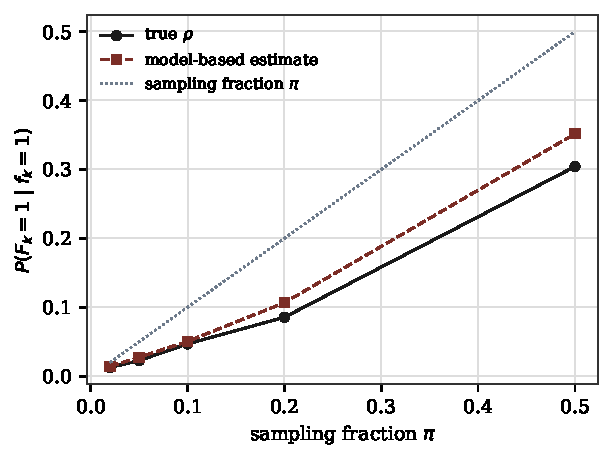
\includegraphics[width=0.66\textwidth]{fig5_journalist.pdf}
\caption{The uniqueness probability $\rho = \Prob(F_k = 1 \mid f_k = 1)$ against the
sampling fraction on the synthetic register: the truth, computed from the known
population; the estimate from a negative binomial law fitted to the sample cell counts;
and the sampling fraction itself, which practice sometimes reports in its place.
Source: the long-form paper, Figure~5.}
\label{c03:fig-journ}
\end{figure}

Naledi's first thought was to put the fitted estimate in the table and stop. Grace asked how the committee would know, on a survey with no census beside it, that the fit was right this time. The synthetic study can answer that question because it knows the truth, and its answer has a second half.

The fit also contains a warning, and it is the more instructive half of the result.
Proposition~\ref{c03:prop-thin} says that the dispersion should not depend on the
sampling fraction, since thinning leaves it unchanged. In the fits it does: the
estimated dispersion rises from 0.33 at $\pi = 0.02$ to 0.51 at $\pi = 0.2$ and 0.59 at
$\pi = 0.5$.
% source: paper/bis_ifc_full.tex lines 1440-1443 (0.33, 0.51); artifacts-paper/results.json (measures.journalist[*].dispersion: 0.325, 0.380, 0.441, 0.505, 0.594)
A parameter that the model says is fixed, drifting steadily with the sampling fraction,
is evidence that the population law is not negative binomial. The estimate of $\rho$ was
still close, because $\rho$ depends mostly on the small classes and the fit gets those
roughly right, but the drift shows that its accuracy rests on the shape of this
particular population. The synthetic study can see the drift because it draws samples
at several fractions from a known population. An institution has one sample, but it can
draw Bernoulli subsamples of that sample at smaller fractions, which by the same
thinning argument are Bernoulli samples of the population at the product fraction, and
fit the model to each. A dispersion that moves across those fits is a reason to report
$\rho$ with the model stated beside it and to treat it as an estimate, which is how
Chapter~15 treats it among its falsification tests.

\section{The table Naledi sent back}

Naledi's revised assessment kept all the numbers and changed the table. Each row now
named the experiment it described: who the adversary was, whether it knew the target
was in the file, whose frequencies were used and whether $\pi$ had been applied. The row
for the uniqueness probability named the fitted model and its dispersion. The row that
multiplied a population-frequency measure by $\pi$ was removed, with a sentence in the
record saying why. Above the table she added the one line the committee would act on:
the declared adversary for the scientific-use file was a prosecutor, so the figure to
compare with the tolerance was the in-file risk, and the other rows were context.

The chair accepted the table and asked for one change. Since the earlier records could
not be reproduced, the committee would treat their tolerances as unowned until each
had been restated against a named experiment. Grace recorded that decision as the
response to her finding.

\section{What each measure answers}

The question of this chapter was what experiment each measure describes and when one
can stand in for another. The answer has three parts.

The measures describe different experiments, and they agree only when the experiments
coincide. The mean prosecutor risk and the in-file marketer risk are one quantity by the
identity of Proposition~\ref{c03:prop-ident}. Every other pair differs by a factor that
the experiment fixes: the inclusion probability separates the in-file figure from the
unconditional one; the ratio of sample to population frequencies separates the
prosecutor's choice among released records from the search of a population list, with a
known sign by Proposition~\ref{c03:prop-plugin}; and the uniqueness probability needs a
model of the population frequencies, without which the sampling fraction is a guess that
was off by a factor of two on the synthetic register.

One figure can therefore stand in for another only when the record shows that the two
experiments are the same, and never by taking the largest. The largest conventional
measure is computed under exact exchangeable matching, and an adversary with
information outside the key is not bound by it. A risk figure is complete when it
states its adversary, whether the target is known to be in the file, which frequencies
it used, whether $\pi$ was applied and, for the journalist, which population model
supplied the frequencies it could not see. With those stated, the figure is no longer
one of several measures. It is the answer to one question, and the next chapter asks
how precisely that answer is known.

\begin{inpractice}\sloppy
Replace the row headed ``re-identification risk'' with one row per declared experiment,
and in each row state the adversary, whether the target is assumed to be in the file,
whether sample or population frequencies were used, and whether the sampling fraction
was applied. Check on any unperturbed release that the mean prosecutor risk equals the
number of distinct released keys divided by the number of released records. Never
multiply a population-frequency measure by the sampling fraction. Do not report the
sampling fraction as a journalist risk. If the uniqueness probability is needed, fit a
population frequency model, state it, and refit it on subsamples of the release to see
whether its parameters hold still.

\smallskip\noindent\textit{In the software.} The checks of Examples~\ref{c3:ex-five} and~\ref{c3:ex-rho} and of Algorithms~3.1 and~3.2 are in \texttt{tests/test\_ext\_measures.py}. The measures are in
\texttt{privacy\_risk.risk}: \texttt{prosecutor\_risk}, \texttt{marketer\_sample\_risk},
\texttt{marketer\_population\_frequency\_risk}, \texttt{marketer\_unconditional\_risk}
and \texttt{journalist\_unique\_probability} for a stated prior on $F_k$. The negative
binomial model is \texttt{FrequencyFit}, fitted by \texttt{fit\_frequency\_model} to the
sample counts of every key cell, zeros included, and evaluated by
\texttt{journalist\_from\_fit}; \texttt{journalist\_truth} computes the target when the
population is known, as in a simulation. The ordering of
Proposition~\ref{c03:prop-plugin} is checked by
\texttt{privacy\_risk.uncertainty.plugin\_ordering}, and
\texttt{privacy\_risk.experiments.conventional\_measures} produces every value in
Figure~\ref{c03:fig-measures}. The uniqueness probability under a fitted law is short
enough to read in full:
\begin{lstlisting}
def journalist_from_fit(pi: float, fit: FrequencyFit) -> float:
    support, mass = fit.probabilities()
    numerator = pi * float(mass[0])
    denominator = float(np.sum(support * pi * (1 - pi) ** (support - 1) * mass))
    return numerator / denominator if denominator else 0.0
\end{lstlisting}
The support starts at one, so the mass at zero is left out of both numerator and
denominator, and it cancels as \eqref{c03:eq-rho} requires.
\end{inpractice}

\begin{mdframed}[linecolor=gray!60,backgroundcolor=gray!5]
\textbf{Algorithm 3.1.} Uniqueness probability under a stated law.\par\smallskip
\textit{Input.} A sampling fraction $\pi$ and a stated law $g$ for the population frequency of a key class, given as probabilities $g(v)$ that sum to one.\par
\textit{Output.} The uniqueness probability $\rho$ of \eqref{c03:eq-rho}.
\begin{enumerate}
\item Refuse the inputs unless $0<\pi\le1$ and the probabilities of $g$ sum to one (to within $10^{-9}$).
\item Form the numerator $N=\pi g(1)$, with $g(1)=0$ when the law puts no mass on one.
\item Form the denominator $D=\sum_{v\ge1}v\pi(1-\pi)^{v-1}g(v)$, the chance that a class leaves exactly one member in the sample, averaged over $g$ (Proposition~\ref{c03:prop-rho}).
\item Return $N/D$, or 0 when $D=0$.
\end{enumerate}
\textit{Checks, each run against the software by the test suite:}
\begin{itemize}
\item The law of Example~\ref{c3:ex-rho} at $\pi=0.1$: 0.0910.
\item The same law at $\pi=0.5$: 0.2667.
\item The same law with the whole population sampled, $\pi=1$: 1.
\item A law with no class of size one, at $\pi=0.1$: 0.
\item A law whose probabilities sum to 0.9: refused.
\item A sampling fraction of zero: refused.
\end{itemize}

\medskip
\textbf{Algorithm 3.2.} Uniqueness probability under a fitted negative binomial law.\par\smallskip
\textit{Input.} The sample counts of the occupied cells of the key space, the number $C$ of cells in the key space, and the sampling fraction $\pi$.\par
\textit{Output.} The fitted population law $\mathrm{NB}(r,\mu)$ and the uniqueness probability $\rho$ under it.
\begin{enumerate}
\item Refuse the inputs if there are more occupied cells than $C$.
\item Add a count of zero for every cell with no released record, so that there are $C$ counts.
\item Fit $\mathrm{NB}(r,m)$ of \eqref{c03:eq-nb} to the $C$ counts by maximum likelihood, searching over $\log m$ and $\log r$ with the Nelder--Mead simplex method, starting from $m$ equal to the mean count (at least $0.001$) and $\log r=0.5$.
\item By Proposition~\ref{c03:prop-thin} the sample law is $\mathrm{NB}(r,\pi\mu)$, so set $\mu=m/\pi$ and keep $r$.
\item Take $g(v)$ as the $\mathrm{NB}(r,\mu)$ probabilities for $v=1,\dots,599$. The mass at zero is left out of numerator and denominator alike, and it cancels as \eqref{c03:eq-rho} requires.
\item Return $\rho=\pi g(1)\big/\sum_{v=1}^{599}v\pi(1-\pi)^{v-1}g(v)$, or 0 when the denominator is zero.
\end{enumerate}
\textit{Checks:}
\begin{itemize}
\item Six occupied cells with counts 3, 1, 1, 2, 5 and 1 in a key space of ten cells, $\pi=0.1$: the fitted population mean, 13 records over 10 cells divided by $\pi$: 13.00.
\item The same counts: $\rho$ under the fitted law: 0.0193.
\item A law with mean 2 and dispersion 0.5, with the whole population sampled: 1.
\item The six occupied cells declared in a key space of four cells: refused.
\end{itemize}
\end{mdframed}

\section{Proofs}

\begin{proof}[Proof of Proposition~\ref{c03:prop-ident}]
By Proposition~\ref{prop:recip}, each released record $i$ has prosecutor risk
$1/f_{K_a(X_i)}$. Group the sum by key value:
\[
\sum_{i \in I}\frac{1}{f_{K_a(X_i)}}
= \sum_{k:\,f_k>0}\ \sum_{i \in I:\,K_a(X_i)=k}\frac{1}{f_k}
= \sum_{k:\,f_k>0} f_k\cdot\frac{1}{f_k}
= \#\{k : f_k > 0\} = D_I .
\]
Dividing by $n$ gives \eqref{c03:eq-ident}.
\end{proof}

\begin{proof}[Proof of Proposition~\ref{c03:prop-plugin}]
By \eqref{eq:freq}, $f_k = \sum_{i\in P} S_i\ind{K_a(X_i)=k} \le
\sum_{i \in P}\ind{K_a(X_i)=k} = F_k$ for every $k$ and every realisation of the
sample, since $S_i \le 1$. For an occupied class, $0 < f_k \le F_k$, so
$1/f_k \ge 1/F_k$ pathwise, and taking expectations preserves the inequality, which is
\eqref{c03:eq-order}. Equality in expectation requires equality almost surely, because
the difference $1/f_k - 1/F_k$ is non-negative; that is, $f_k = F_k$ for every class
the average touches, so every population member of each such class is sampled.

For \eqref{c03:eq-jensen}, the function $x \mapsto 1/x$ is strictly convex on
$(0,\infty)$. Jensen's inequality for a random variable that is positive with
probability one and has finite mean gives $\E[1/f_k] \ge 1/\E[f_k]$, with equality if
and only if $f_k$ is almost surely constant.
\end{proof}

\begin{proof}[Proof of Proposition~\ref{c03:prop-rho}]
Under Bernoulli sampling with common probability $\pi$, the sample frequency of a class
with $F_k = v$ members is a sum of $v$ independent Bernoulli($\pi$) indicators, so
$f_k \mid F_k = v \sim \mathrm{Binomial}(v,\pi)$ and
$\Prob(f_k = 1 \mid F_k = v) = v\pi(1-\pi)^{v-1}$. A class with $f_k = 1$ has
$F_k \ge 1$. Bayes' theorem gives
\[
\rho_k = \frac{\Prob(f_k = 1 \mid F_k = 1)\,g(1)}
{\sum_{v\ge1}\Prob(f_k=1\mid F_k=v)\,g(v)}
= \frac{\pi\,g(1)}{\sum_{v\ge1}v\pi(1-\pi)^{v-1}g(v)},
\]
which is \eqref{c03:eq-rho}. For \eqref{c03:eq-journ}, note that
$1/F_k \ge \ind{F_k = 1}$ whenever $F_k \ge 1$, since the left side equals the right
side when $F_k = 1$ and is positive otherwise. Taking conditional expectations given
$f_k = 1$ gives $\E[1/F_k \mid f_k = 1] \ge \Prob(F_k = 1 \mid f_k = 1) = \rho_k$, with
equality only if $\Prob(F_k \ge 2 \mid f_k = 1) = 0$.
\end{proof}

\begin{proof}[Proof of Proposition~\ref{c03:prop-thin}]
Use probability generating functions. With $p = r/(r+\mu)$, the generating function of
$\mathrm{NB}(r,\mu)$ is
\[
G_F(s) = \E[s^F] = \Big(\frac{p}{1-(1-p)s}\Big)^{r}
= \Big(1 + \frac{\mu}{r}(1-s)\Big)^{-r}, \qquad |s| \le 1 .
\]
Given $F$, $f$ is a sum of $F$ independent Bernoulli($\pi$) variables, whose common
generating function is $1-\pi+\pi s$. Hence
\[
G_f(s) = \E\big[\E[s^f \mid F]\big] = \E\big[(1-\pi+\pi s)^F\big]
= G_F(1-\pi+\pi s)
= \Big(1 + \frac{\mu}{r}\,\pi(1-s)\Big)^{-r},
\]
which is the generating function of $\mathrm{NB}(r,\pi\mu)$. A generating function on
$|s|\le 1$ determines the law, so $f \sim \mathrm{NB}(r,\pi\mu)$.

For identification, the $C$ sample cell counts are then independent draws from
$\mathrm{NB}(r,\pi\mu)$. The negative binomial family is identified in its parameters:
its mean is $\pi\mu$ and its variance is $\pi\mu + (\pi\mu)^2/r$, so the first two
moments of the count law determine $\pi\mu$ and $r$ uniquely. Since $\pi$ is known,
$\mu$ follows, and with it the population law $\mathrm{NB}(r,\mu)$ of every cell. The
maximum likelihood estimator of $(r,\pi\mu)$ from the $C$ counts is consistent as
$C \to \infty$ under the usual regularity conditions for this family
\citep{vandervaart1998}.
\end{proof}
